\section{分层架构、数据流与责任边界}
\label{sec:architecture}
\subsection{从源码到事实，再从事实到结论}
应用层负责确定本次运行范围、选择能力、调度确定性工作并交付结果。源码适配器把原始文件变成带符号和绑定信息的文档；索引和检索负责可见范围。工具负责产出受信类型化观察。准入和归并负责判断这些观察是否支持声明性质。presentation 只呈现既有结果，不重新分析源码，也不补充证明。

研究路径中的模型负责提出取证动作和解释观察，不能选择自己的源码摘要、替换运行时策略或把自己写的状态字符串当作工具证明。评价侧拥有标签和统计职责；它不把映射回流到候选 ID、路径别名或模型提示。

\begin{figure}[htbp]\centering
\begin{tikzpicture}[node distance=6mm and 10mm]
\node[wide] (source) {显式授权源目录\\源码边界读取 / 原始字节摘要};
\node[wide,below=of source] (index) {文档 + 符号 + 调用关系\\确定性候选与作用域准入};
\node[box,below=of index,xshift=-41mm,fill=green!7,draw=green] (static) {应用服务\\静态能力 + 有限任务控制};
\node[box,below=of index,xshift=41mm,fill=warm!8,draw=warm!80!black] (research) {研究编排\\Code-RAG / Jev / ReAct};
\node[wide,below=30mm of index] (tools) {共享工具边界\\参数、subject、调用记忆、预算与投递};
\node[box,below=of tools,xshift=-41mm,fill=green!7,draw=green] (reduce) {产品归并\\事实集合 $\rightarrow$ 性质状态};
\node[box,below=of tools,xshift=41mm,fill=warm!8,draw=warm!80!black] (votes) {研究准入 + 投票\\最终实质票重新检查};
\node[wide,below=31mm of tools] (output) {JSON / 人工报告 / 原始观察 / 用量\\评价与研究门槛独立判断};
\draw[arrow] (source)--(index);\draw[arrow] (index)--(static);\draw[arrow] (index)--(research);
\draw[arrow] (static)--(tools);\draw[arrow] (research)--(tools);
\draw[arrow] (tools)--(reduce);\draw[arrow] (tools)--(votes);
\draw[arrow] (reduce)--(output);\draw[arrow] (votes)--(output);
\end{tikzpicture}
\caption{修后总体数据流。应用与研究路径共享源、工具与证据契约，但产品不等待模型 quorum。原始产物、公开投递和最终判断是不同记录面。}
\label{fig:architecture_current}
\end{figure}

\subsection{源码包的实际分工}
\begin{longtable}{L{29mm}rL{112mm}}
\caption{当前 Python 包规模与职责。数量由源码清单计算，含各包初始化文件。}\label{tab:packages}\\
\toprule 包 & 文件 & 主要职责\\\midrule\endfirsthead
\caption[]{（续）}\\
\toprule 包 & 文件 & 主要职责\\\midrule\endhead
\code{application} & 9 & 产品预检、服务、控制、身份、上下文授权、投递预算和确定性归并。\\
\code{presentation} & 2 & 从 ReviewResult 渲染报告和原子提交，不承载分析器。\\
\code{domain} & 7 & 源、证据、计划、对话、研究判断和产品契约的数据模型。\\
\code{agents} & 12 & 发现、规划、Jev、ReAct、适用性、投票和共享观察记账。\\
\code{code_adapters} & 11 & Python、Java、Go、JS/TS 的 AST/词法适配及边界读取。\\
\code{retrieval} & 6 & 文档索引、词法/BM25、图关系、上下文和计量。\\
\code{tools} & 26 & 工具注册；有界命令/数据流/权限/eval 分析及验证适配。\\
\code{runtime} & 27 & 模型传输、门禁、预算、日志、快照、隔离和 witness 内核。\\
\code{harness} & 7 & 系统、专家、预算、命令及结果的一致性规范。\\
\code{baselines} & 14 & 保留的确定性 V 系列和诊断对照。\\
\code{evaluation} & 107 & 数据组合、环境准备、runner、诊断、指标、生命周期和 readiness。\\
顶层 & 2 & 包初始化和 CLI。\\\bottomrule
\end{longtable}

\begin{figure}[htbp]\centering
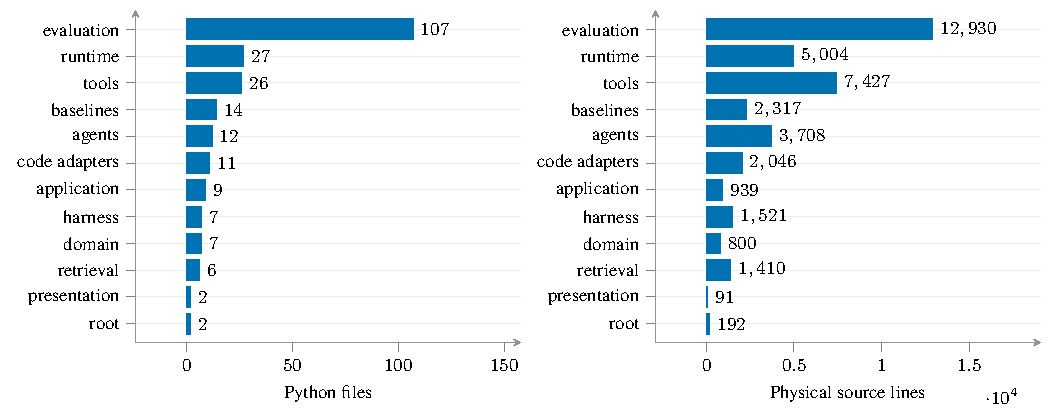
\includegraphics[width=\textwidth]{figures/code_footprint.pdf}
\caption{代码结构的描述性清点：230 文件、38385 物理行。evaluation 的文件数最多；这说明历史实验基础设施占比，不意味着相同语义覆盖、质量或用户价值。行数包含注释和空行。}
\label{fig:footprint}
\end{figure}
\source{data/report_data.json; src/cv_agent/**/*.py}

\subsection{核心与评价的依赖隔离}
K2 已把 witness 内核迁入 \code{runtime/witness/}，契约、读取政策、追踪、资源计数、场景运行及义务分别在同一包中。生产工具依赖运行时；准备器、runner 和诊断依然归 evaluation。核心 \code{agents/tools/runtime} 不反向导入评价包；新产品的公共 CLI 子命令采用延迟导入，产品测试显式拒绝导入 evaluation。

架构边界检查覆盖显式、嵌套、类型检查和已列出的字面动态导入；它不穷尽任意生成的 import 字符串。K2 的归一化文本/AST、源码绑定及实际结果对照属于迁移验收，不能替代新产品的端到端验收。\cite{k2,acceptance}

\subsection{契约作为层间接口}
\code{Candidate} 和 \code{ValidationSubject} 建立问题对象；\code{ToolObservation} 建立产出身份；\code{AgentExpertVote} 表达研究判断；\code{ReviewResult} 表达产品交付。中间过程不能用一个自然语言状态覆盖这些职责。控制器可以判定“操作完成”，但语义内核仍可以判定 UNKNOWN；报告可成功交付，而 run 可以是 PARTIAL 或 BLOCKED。
\loc{application/; presentation/report.py; domain/; agents/workflow.py}
